\chapter{Marco te\'orico}

\section{PBR}
PBR o \textit{physically based rendering} es el t\'ermino que se utiliza para nombrar al grupo de t\'ecnicas basados en un
modelo f\'isico. La intenci\'on es conseguir aproximaciones r\'apidas y plausibles de la interacci\'on de un flujo de luz
con una superficie. Las principales ventajas de este tipo de algoritmos son la consistencia bajo diferentes condiciones de
luz y su manejo intuitivo por parte de los artistas.
Los motores PBR cumplen con la ley de la conservaci\'on de la energ\'ia y utilizan BRDFs basados en la teor\'ia de
microfacetas. Adicionalmente, otros elementos de la escena, como la c\'amara o las luces, pueden estar basados en modelos
f\'isicos para ofreciendo para aumentar el grado de realismo.

\section{Ecuaci\'on de render}
El prop\'osito de la ecuacion de render es conocer el valor de radiancia que llega a la camara en una direcci\'on
por cada pixel  de la camara.

Para saber la radiancia sobre un punto en una direcci\'on, utilizamos la ecuacion de reflectancia, que depende
de la luz que llega al puntos, el coseno del angulo con el que incide la luz y el BRDF (bidirectional reflectance
distribution function), que modela el comportamiento de la luz al rebotar sobre la superficie.\\

\begin{eqfloat}[!htb]
    \begin{equation}
        L_o(p, w_o) = L_e(x, w_o) + \int_\Omega{f_r(p, w_i, w_o) L_i(p, w_i) n\cdot{w_i}dw_i}
    \end{equation}
  \caption{Ecuaci\'on de render}
\end{eqfloat}
\singlespacing

Siendo $L_o(p, w_o)$ la luz reflectada por la superficie, $L_e(x, w_o)$ la luz emitida por la superficie, que est\'a fuera
de la integral porque es independiente de la luz reflejada o refractada por la superficie. $\int_{\Omega}[...]dw$ que representa
que la operaci\'on se repite para cada \'angulo s\'olido dentro de la semiesfera $f_r(p, w_i, w_o)$ el BRDF $L_i(p, w_i)$ la luz
que llega al punto de la superficie que estamos evaluando $n\cdot{w_i}$ el factor de atenuaci\'on de la luz con respecto a la normal.

\section{BRDF}

El BRDF, o función de ditribuci\'on bidireccional de reflectividad, es la parte de la ecuaci\'on que describe el
comportamiento de la luz al golpear sobre la superficie y se utiliza para rmodelar propiedades f\'isicas de los diferentes
materiales. Es una funcion estad\'istica que calcula cuanta de la luz que incide sobre un material es reflejada en direcci\'on
a la c\'amara, o, en otras palabras, para ello toma como argumentos la direccion de la luz, $w_i$, y la dirección de salida,
$w_o$, la normal de la superficie, n, y un par\'ametro $\alpha$ que representa la rugosidad del material.

\begin{figure}[H]
    \vspace{0.5cm}
    \centering
      \frame{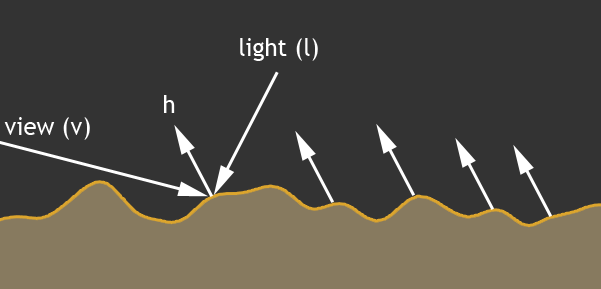
\includegraphics[scale=0.7]{microfacet-diagram}}
    \caption{Diagrama de la luz incidente y luz reflectada}
    \vspace{0.5cm}
\end{figure}

Para que un BRDF se considere como PBR, ha de utilizar el modelo de microfacetas, ademas de cumplir con la ley de conservacion
de la energia, $\forall w_i \int_{\Omega} f(p, w_i, w_o) n\cdot{w_i} dw_o \leq 1$ y el principio de reciprocidad de Helmholtz,
el BRDF debe de ser simétrico, esto es que invertir la direccion de entrada y salida del BRDF no deberia afectar al resultado
$f(x, w_i, w_o) = f(x, w_o, w_i)$ sin embargo, los motores en tiempo real, frecuentemente incumplen el principio de reciprocidad,
no siendo fisicamente plausibles, pero sin generar artefactos.\\

    \subsection{Teor\'ia de microfacetas}

    \bgroup

        Aunque a escala macrosc\'opica podamos considerar una superficie como lisa, ninguna superficie es completamente lisa a nivel
        microsc\'opico. La teor\'ia de microfacetas utiliza una representaci\'on estad\'istica para modelar estas peque\~nas irregularidades.
        Para ello, la teor\'ia de microfacetas, considera la superficie de reflexi\'on como una superficie compuesta por una matriz de
        superficies mas peque\~nas que la longitud de onda de la luz pero muy peque\~nas desde el punto de vista de la c\'amara,
        completamente reflectantes, llamadas microfacetas, y cuyas diferentes orientaciones determinan la rugosidad de la superficie.
        Si las microfacetas est\'an completamente alineadas, las reflexiones ser\'an mas definidas, asimilandose a un espejo, mientras
        que las microfacetas apuntando en diferentes direcciones, daran como resultado una reflexion especular mas difusa.

        \begin{figure}[H]
            \vspace{0.5cm}
            \centering
            \frame{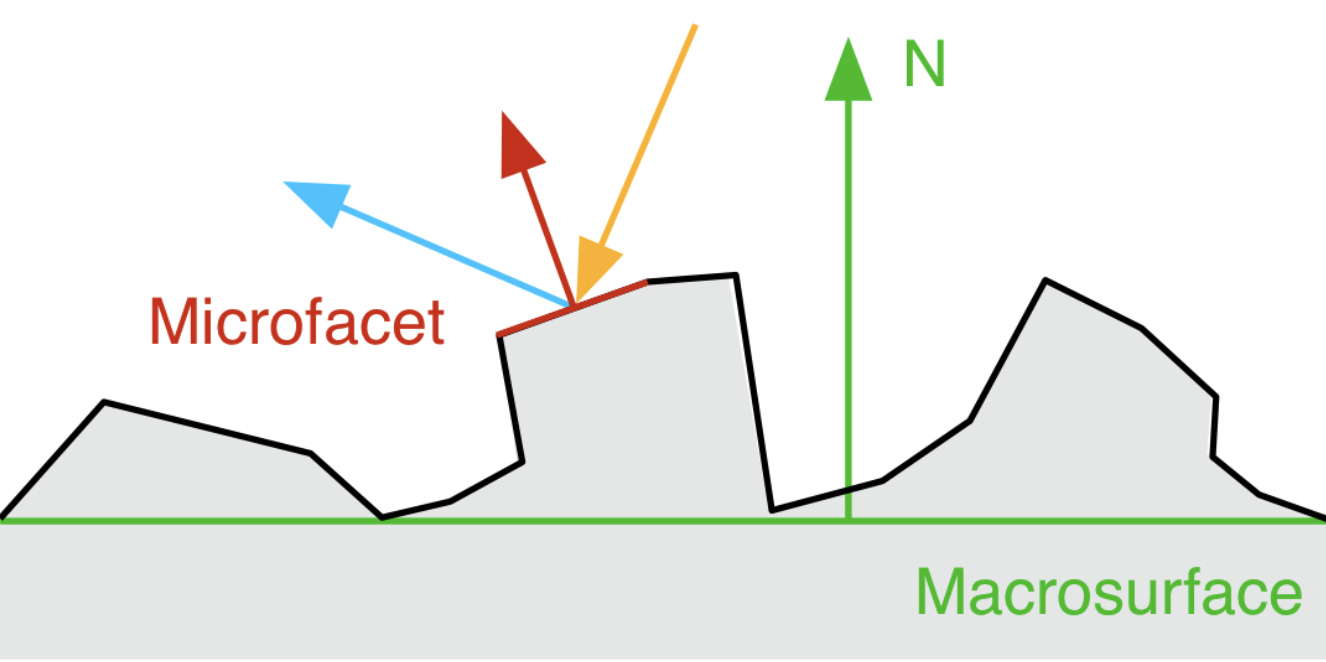
\includegraphics[scale=0.55]{macrosuperficie}}
            \caption{Superficie a escala microsc\'opica}
            \vspace{1.0cm}
        \end{figure}

    \egroup


    \subsection{Tipos de BRDFs}
    Los diferentes tipos de BRDFs permiten para modelar diferentes propiedades de los materiales, isotropia o anisotropia,
    transmitancia, reflexiones internas, etc. Podemos clasificar los diferentes tipos de BRDFs entre modelos analiticos y BDRFs
    de datos adquiridos. Los modelos analiticos son funciones matemáticas que modelan diferentes efectos de la luz en funcion de
    sus datos de entrada, mientras que los BRDFs de datos adquiridos, capturan el BRDF de un material con un gonioreflectometro,
    y permiten una representacion muy precisa del material escaneado.

    Comunmente, en la industria se utilizan modelos anal\'iticos, debido a su flexibilidad y rendimiento y el mas utilizado a
    d\'ia de hoy en la industria, aunque con algunas variaciones en sus t\'erminos, sigue siendo el modelo de Cook-Torrance\autocite{cooktorrance}.
    \todo[inline]{
        Metal. The appearance of the metal mainly depends on the direct reflection of light at the interface of the two media (ie, specular reflection). The metallic specular reflection color is a three-channel color, and R, G, and B are different. The light refracted into the metal is almost immediately absorbed by free electrons, and there is no scattering of light refracted into the metal.
        Non-Metal. Non-metal is a dielectric, and its overall appearance is mainly determined by its combination of absorption and scattering characteristics. Similarly, the interaction between non-metal and light is divided into reflection and refraction. According to the scattering and absorption characteristics of the medium type, refraction is divided into multiple categories:
    }
    \todo[inline]{
        The term isotropic is used to describe BRDFs that represent reflectance properties that
        are invariant with respect to rotation of the surface around the surface normal vector.
        Consider a small relatively smooth surface element and fix the light and viewer positions.
        If we were to rotate the surface about its normal, the BRDF value (and consequently the
        resulting illumination) would remain unchanged. Materials with this characteristic such
        as smooth plastics have isotropic BRDFs.
        Anisotropy, on the other hand, refers to BRDFs that describe reflectance properties that
        do exhibit change with respect to rotation of the surface around the surface normal
        vector. Some examples of materials that have anisotropic BRDFs are brushed metal,
        satin, and hair. In general, most real-world BRDFs are anisotropic to some degree, but
        the notion of isotropic BRDFs is useful because many classes of analytical BRDF models
        fall within this class. In general, most real-world BRDFs are probably more isotropic
        than anisotropic though many real-world surfaces have subtle anisotropy. Any material
        that exhibits even the slightest anisotropic reflection has a BRDF that is anisotropic. 
    }

    \begin{figure}[H]
        \centering
        \frame{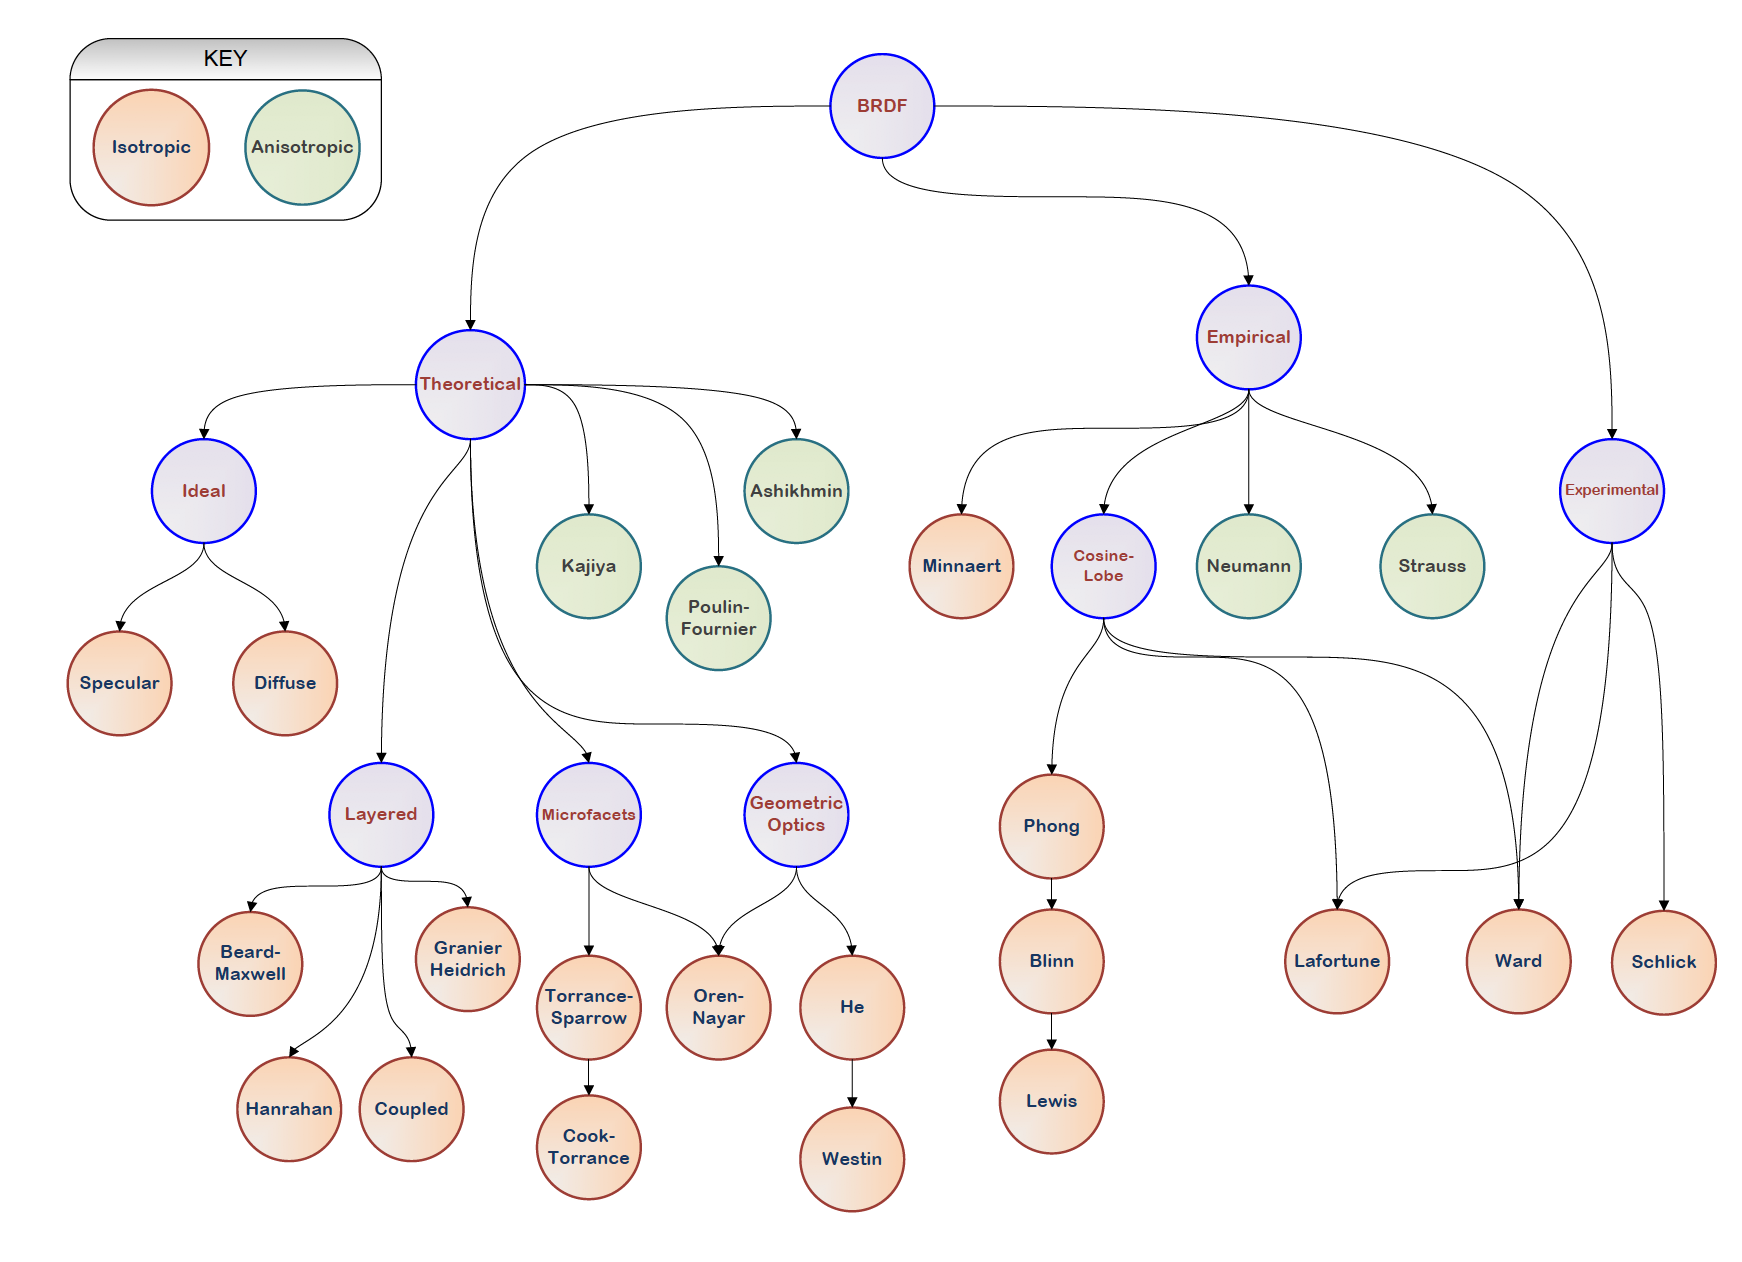
\includegraphics[scale=0.45]{schema_brdfs}}
        \caption{Esquema de diferentes modelos de BRDF seg\'un su origen}
        \vspace{0.5cm}
    \end{figure}

    \section{Limitaciones de los motores de renderizado en tiempo real}
    Los motores de renderizado en tiempo real deben utilizar algoritmos lo menos costosos posibles para garantizar un buen
    tiempo de respuesta. Es por ello que sus BRDFs, pueden ser m\'as sencillos que los implementados en sistemas de \textit{path-tracing},
    ofreciendo una soluci\'on de compromiso entre el rendimiento y los fen\'omenos f\'isicos representados por el modelo.\\
    
    Por otra parte, resolver la parte integral de la ecuaci\'on de render:

    \begin{center}$L_o(p, w_o) = \int_{\Omega} f_r(p, w_i, w_o)L_i(p, w_i)n\cdot{w_i}dw_i$\end{center}
    \singlespacing
    requiere lanzar rayos no en una direcci\'n si no desde todas las posibles direcciones sobre la semiesferea $\Omega$, por
    lo que no es posible en tiempo real, sin embargo, m\'as adelante analizaremos t\'ecnicas que p\'ermiten simular \'este
    efecto utilizando c\'alculos precomputados o aproximando la soluci\'on de forma anal\'itica.\\


